\section{Einzelne Entscheidungsbäume}
\label{sec:dt_ind_decision_trees}
Der einzelne Entscheidungsbaum ist eine rekursive Datenstruktur um Entscheidungsregeln darzustellen \cite{quinlan1990decision}.
Jeder innere Knoten ist ein \textit{Test}, welcher eine arbiträre Anzahl von sich gegenseitig auschließenden Ergebnissen hat.
Das Ergebnis eines Tests bestimmt mit welchem Kindknoten fortgefahren wird.
Die Blätter des Baumes stellen die Entscheidungen dar bzw. die Klassen des Entscheidungsbaumklassifizierers.
Abbildung \ref{fig:entscheidungsbaum} zeigt einen binäreren Entscheidungsbaum, in dem jeder Test zwei mögliche Ergebnisse hat.
\begin{figure}[h!]
    \centering
    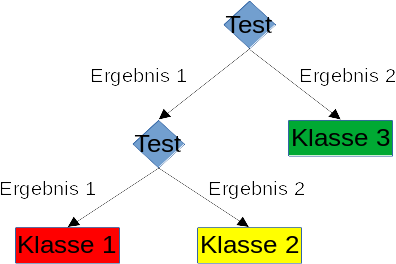
\includegraphics[width=0.5\linewidth]{images/entscheidungsbaum.png}
    \caption{Beispiel eines binären Entscheidungsbaums mit 3 möglichen Ergebnissen.}
    \label{fig:entscheidungsbaum}
\end{figure}
Das Trainieren von Entscheidungsbäumen ist eine Art von \textit{Supervised Learning}, d. h. aus einer beschrifteten Trainingsmenge werden Regeln abgeleitet, um das korrekte Mapping von Input
zu Output abzubilden \cite{goshKMeans}. Die Trainingsmenge besteht aus Feature-Mengen, die mit Klassen beschriftet sind \cite{steinbergCART}. Die Generalisierungsfähigkeit ist abhängig von der
Trainingsmenge. Zum einen sollte die Trainingsmenge möglichst repräsentativ sein für die Aufgabe, die gelernt werden soll. Zum anderen sollten die verwendeten Features eine Partitionierung
aller Klassen ermöglichen \cite{pei1998feature}.
\newline
\newline
Entscheidungsbäume werden heuristisch konstruiert, da die Konstruktion eines optimalen Entscheidungsbaumes NP-Vollständig ist \cite{laurent1976constructing}. Zu diesen Algorithmen gehören
beispielsweise \texttt{ID3} \cite{quinlan1986induction}, \texttt{C4.5} \cite{quinlan2014c4} oder \texttt{CART} \cite{breiman1984classification}. Die Aufgabe ist durch gezielte Trennungen
eine Partitionierung der Trainingsmenge zu erzeugen, sodass möglichst nur Einträge mit der gleichen Beschriftung in einer Partitionierung enthalten sind. Die Algorithmen unterscheiden
sich in ihrer Strategie \cite{quinlan1986induction}.
\newline
\newline
Scikit-Learn implementiert eine optimierte Version des \textit{CART} (\textbf{C}lassification \textbf{A}nd \textbf{R}egression \textbf{T}rees) Algorithmus \cite{ScikitLearnCART}.
CART partitioniert die Trainingsmenge indem lokal immer die beste Teilung ausgewählt wird, d. h. es wird für die momentane Teilmenge immer die beste Teilungsregel ausgewählt.
Dieser Vorgang wird rekursiv mit jeder Teilmenge wiederholt, bis keine weitere Teilung mehr möglich ist oder alle Einträge einer Partitionierung die gleiche Beschriftung tragen \cite{steinbergCART}.